
\section{Signals and properties}

\subsection{Properties of analog signals}

\paragraph{Analog signal} We define a signal is this course as a function of
time or space. For instance $x:\R\rightarrow\dbC$ is a complex 1D signal of time
$t\in\dbR$. $x:\R^2\rightarrow\dbR$ is a 2D image of space $\p\in\dbR^2$.

\paragraph{Causality}\index{Causal signal}
A signal $x(t)$ is causal if 
$$ x(t)=0,\quad \forall x<0 $$

Example: $x(t)= \begin{cases}
0& \text{for } t<0\\
\sin(t)\exp\left(-\frac{t^2}{2}\right) & \text{for } t\geq 0
\end{cases}$

\paragraph{Periodicity}\index{Periodic signal}
A signal $x(t)$ is periodic of period $T_0$ is
$$x(t-kT_0)=x(t),  \forall t\in\mathbb{R}, \forall k\in\mathbb{N}$$      


Example: $x(t)= %\begin{cases}
 % \exp(-\frac{(t-1)^2}{2})&  0<t<T\\
  \exp\left(-\frac{(t-kT_0-1)^2}{2}\right)  \text{ for }kT_0<t<(k+1)T_0,\quad
  \forall k\in\mathbb{N}$
  
\begin{figure}[t]
    \centering
    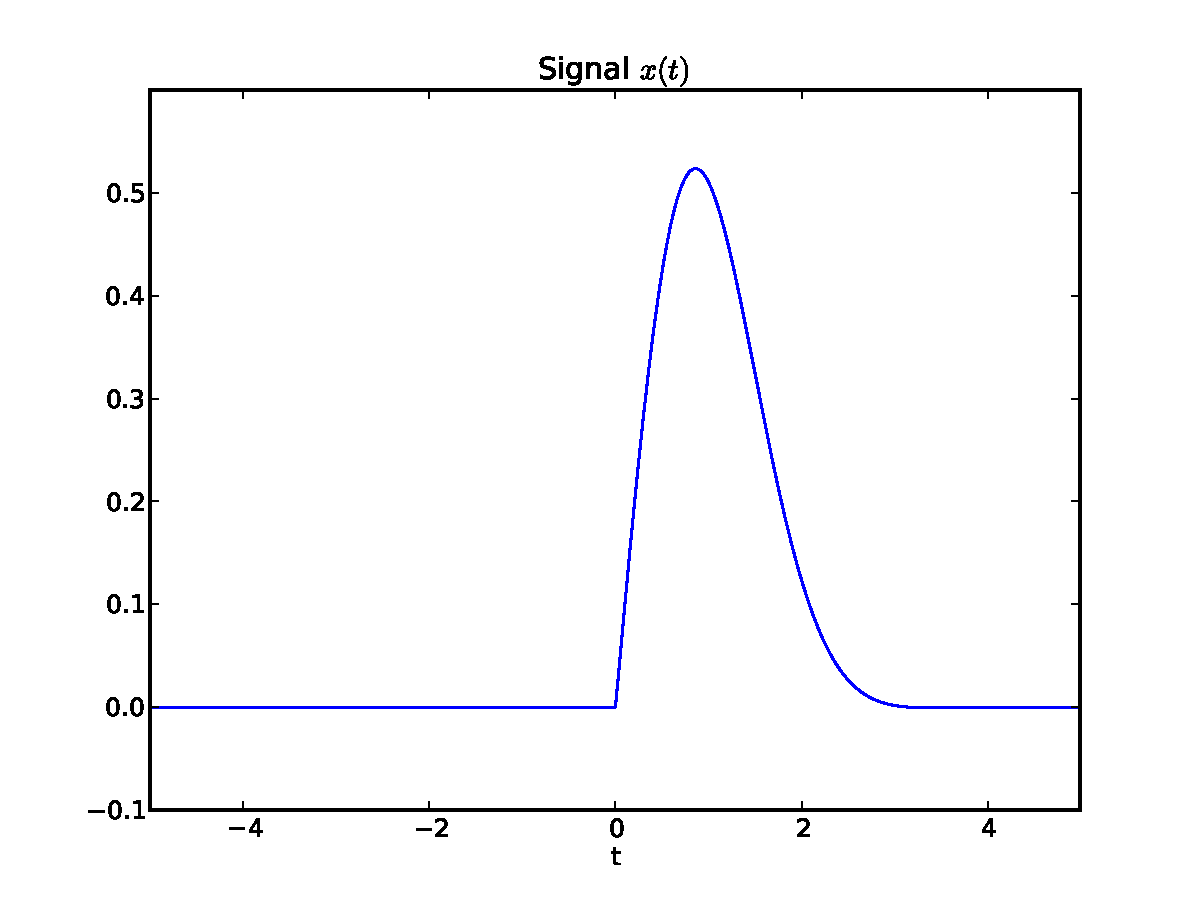
\includegraphics[width=.45\linewidth]{imgs/sig_conv/sig_causal.pdf}
    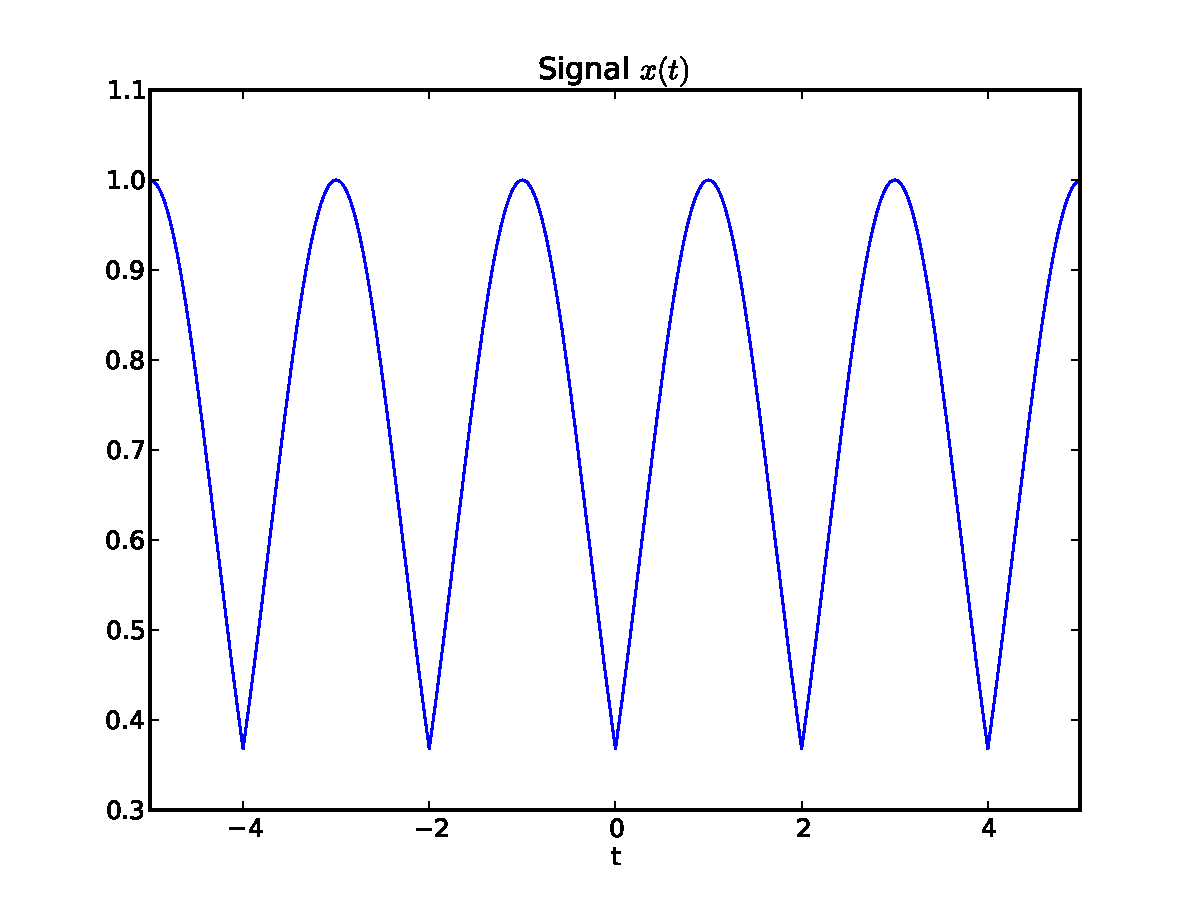
\includegraphics[width=.45\linewidth]{imgs/sig_conv/sig_per.pdf}
    \caption{Examples of Causal signal (left) and periodic signal (right).}
    \label{fig:ex_causal_per}
\end{figure}



\paragraph{Signal in $L_p$ space}\index{$L_p$ space}
$L_p(S)$ is the set of functions whose absolute value to the power of $p$
has a finite integral or equivalently that
\begin{equation}
  \|x\|_p=\int_S |x(t)|^p dt < \infty
  \label{eq:lp_space}
\end{equation}
\begin{itemize}
  \item $L_1(\dbR)$ is the set of absolute integrable functions
  \item $L_2(\dbR)$ is the set of quadratically integrable functions (finite energy)
  \item $L_\infty(\dbR)$ is the set of bounded functions
\end{itemize}

\paragraph{Instantaneous power}\index{Power}
The instantaneous power of signal $x(t)$ 
\begin{equation}
  \label{eq:puissinst}
  p_x(t)=|x(t)|^2
\end{equation}
 Unit :  Watt (W).


 \begin{block}{Energy of a signal}\index{Energy}
  We define the energy of a signal $x(t)$ as :
\begin{equation}
\label{eq:enerfinie}
E=\pause \int_{-\infty}^{+\infty}|x(t)|^2dt
\end{equation}
the signal is said to be of finite energy if $E<\infty$ ($\|x\|_2<\infty$ means $x\in L_2(\dbR)$).

Unit: Joule, Calorie or Watt-hour (J, Cal ou Wh, 1 calorie = 4.2 J).
\end{block}

\begin{block}{Average power of a signal}
  
  The average power of a signal is defined as
   \begin{equation}
     \label{eq:puissance}
    P_m= \pause\lim_{T\rightarrow\infty} \frac{1}{T}\int_{-\frac{T}{2}}^{+\frac{T}{2}}|x(t)|^2dt
   \end{equation}
   \begin{itemize}
   \item For a periodic signal, the average power can be computed on a unique period.
   \item Power is homogeneous to an energy divided by time.
   \item $P_{RMS}=\sqrt{P_m}$ is called the Root Mean Square power ("valeur efficace" in french).
   \item A finite energy signal has a n average power $P_m=0$.
   \item  Unit :  Watt (W).
   \end{itemize}
   
     \end{block}


     \begin{block}{Additive noise}
      Additive noise is a kind of noise that is added to the signal of interest.
  $$y(t)=x(t)+b(t)$$
  $y(t)$ is the observed signal, $x(t)$ the signal of interest and
  $b(t)$ is the noise.
    \end{block}

    \begin{block}{Signal-to-Noise ratio (SNR)} \index{SNR}\index{Signal-to-Noise ratio}
      The Signal to Noise Ratio is defined as:
  \begin{equation}
    \label{eq:rsb}
    SNR=\frac{P_S}{P_N} \quad \text{ ou } \quad SNR(dB)=10\log_{10}(SNR)
  \end{equation}
  where $P_S$ is the power of the signal and $P_N$ the power of the noise.
  \begin{itemize}
  \item An Analog-to-Digital conversion process should have the best possible SNR.
  \item The SNR is often used for additive noise models.
  \item Other measures such as Peak Signal to Noise Ratio (PSNR) can be used on specific data (images).
  %\item Le RSB est également appelé SNR pour Signal to Noise Ratio.
  %\item Le Rapport signal sur signal + bruit est également utilisé.
  %$$ R_{S/S+B}=\frac{P_S}{P_{S+B}}$$
  \item One of the objective of filtering is to get a better SNR when the signal and the noise have different frequency contents..
  \end{itemize}
    \end{block}





\subsection{Common signals}
\label{sec:common_sig}


\begin{block}{Heaviside function}
  \begin{equation}
\label{eq:heaviside}
\Gamma(t)=
\begin{cases}
  0& \text{if } t<0\\
  1/2& \text{if } t=0\\
  1 & \text{if } t>0
\end{cases}
\end{equation}
%Exemple: On allume une ampoule.
Also known as the step function.
\end{block}

\begin{block}{Rectangular function}
  \begin{equation}
   \Pi_T (t)=
   \begin{cases}
     1/T& \text{if } |t|< T/2\\
     1/2T& \text{if } |t|= T/2\\
     0& \text{else}
   \end{cases}
   \label{eq:rectangular}
 \end{equation}
 %\vspace{-.5cm}
 \begin{itemize}
 \item $\Pi(t)=\frac{1}{T}(\Gamma(t-\frac{T}{2})-\Gamma(t+\frac{T}{2}))$.
 \item Finite energy signal (finite support).
 \end{itemize}
   \end{block}


   \begin{block}{Complex exponential }
    let $e_z(t)$ be the following function $\dbR \rightarrow \dbC$
 \begin{equation}
   \label{eq:expcomplexe}
   e_z(t)=\exp(zt)
 \end{equation}
 where $z$ is a complex number.
 When $z=\tau+wi$ the, 
 \begin{equation*}
   \label{eq:expcomplexe2}
   e_z(t)=(\cos(wt)+i\sin(wt))\exp(\tau t)
 \end{equation*}
 %\vspace{5mm}
 
 
 Special cases:
 \begin{itemize}
 \item $z=\tau$ real, then we recover the classical exponential.
 $$e_z(t)=\exp(\tau t)$$
 
 \item $z=wi$ imaginary then
 $$e_z(t)=\cos(wt)+i\sin(wt) $$
 
 % \item $z=\tau+wi$ quelconque alors
 %   $x(t)=(\cos(w*t)+i*\sin(w*t))\exp(\tau t)$
 \end{itemize}
   \end{block}

\begin{figure}[ht]
  \centering
  \begin{tabular}{|c|ccc|}\hline
    $\tau \backslash w$ & $-2$ & $0$ & $2$ \\\hline
   \raisebox{9mm}{$-0.5$} 
    & 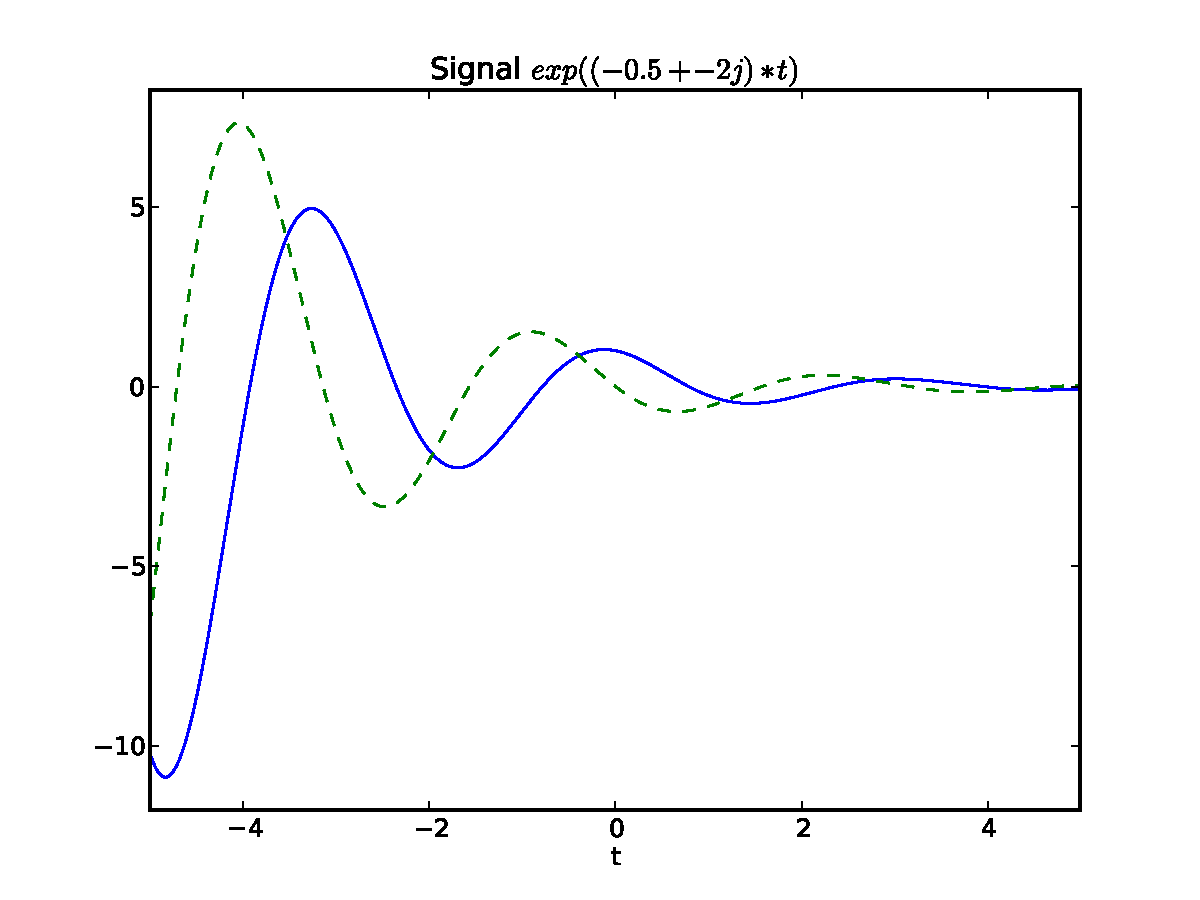
\includegraphics[width=.25\linewidth]{imgs/sig_conv/sig_exp-1-1.pdf}
    & 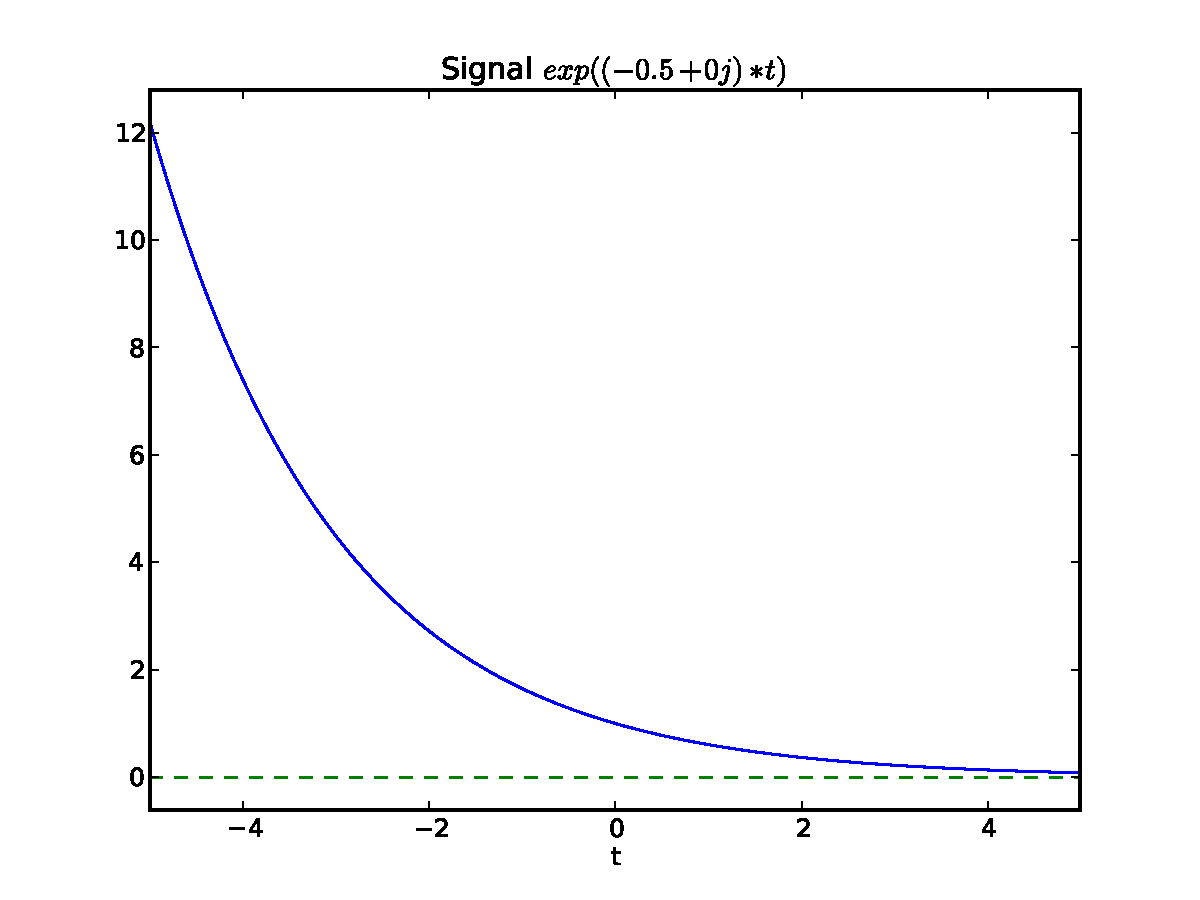
\includegraphics[width=.25\linewidth]{imgs/sig_conv/sig_exp-10.pdf}
    & 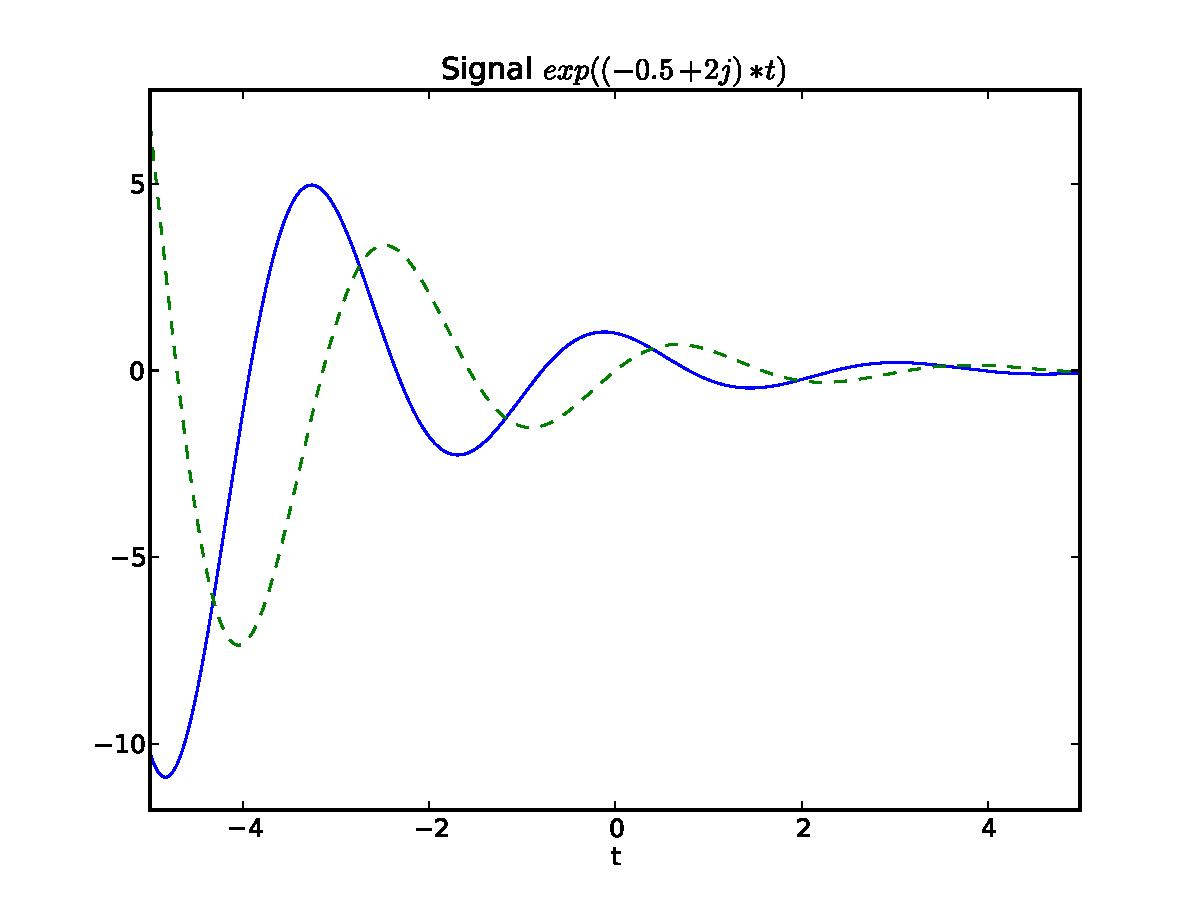
\includegraphics[width=.25\linewidth]{imgs/sig_conv/sig_exp-11.pdf}\\
   \raisebox{9mm}{$0$} 
    & 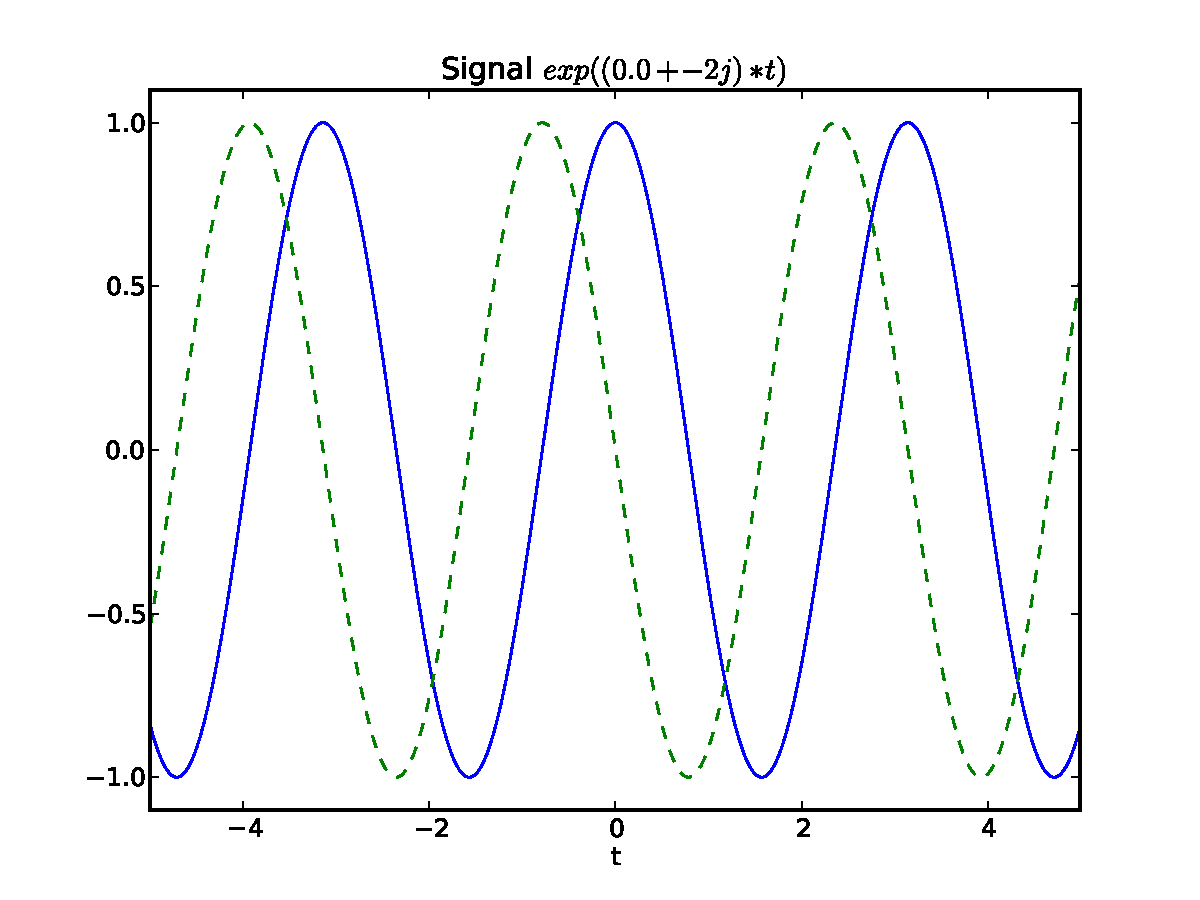
\includegraphics[width=.25\linewidth]{imgs/sig_conv/sig_exp0-1.pdf}
    & 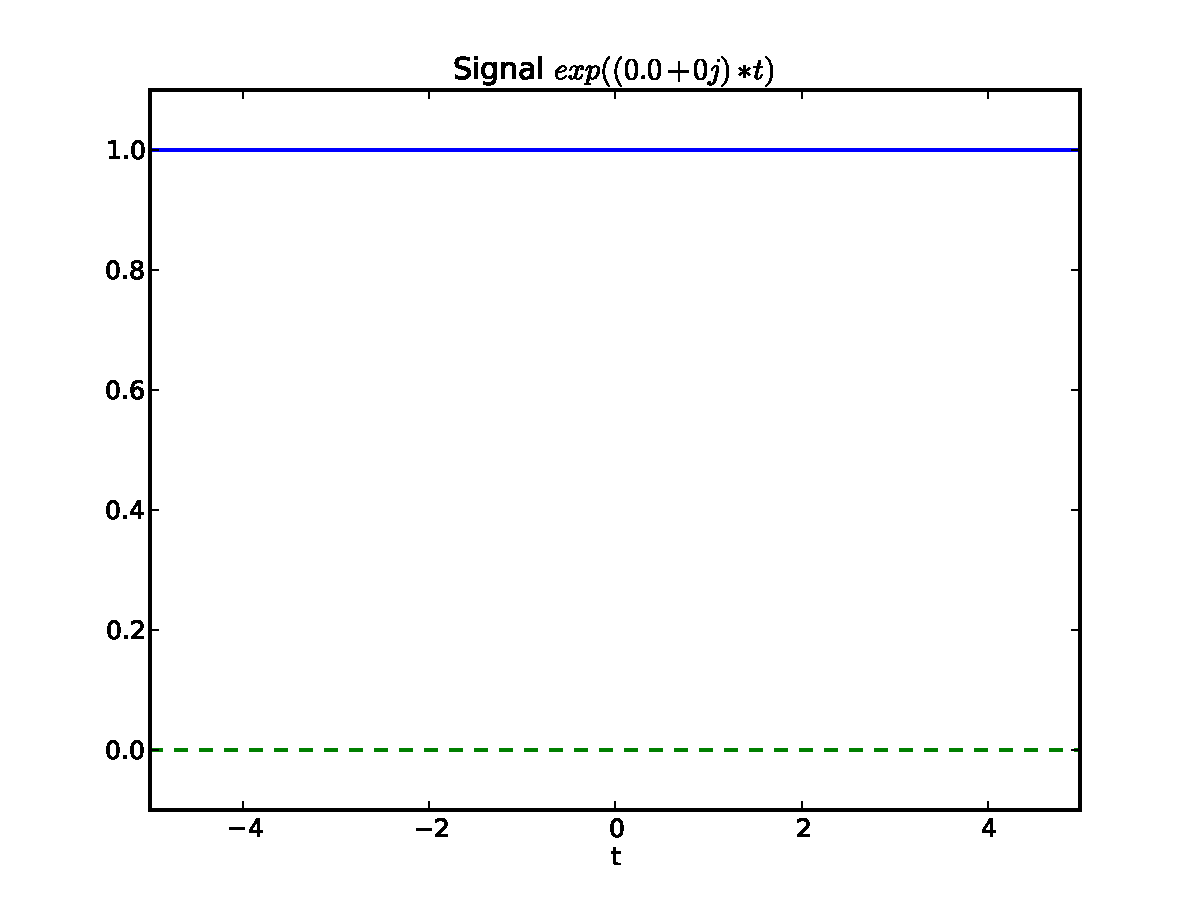
\includegraphics[width=.25\linewidth]{imgs/sig_conv/sig_exp00.pdf}
    & 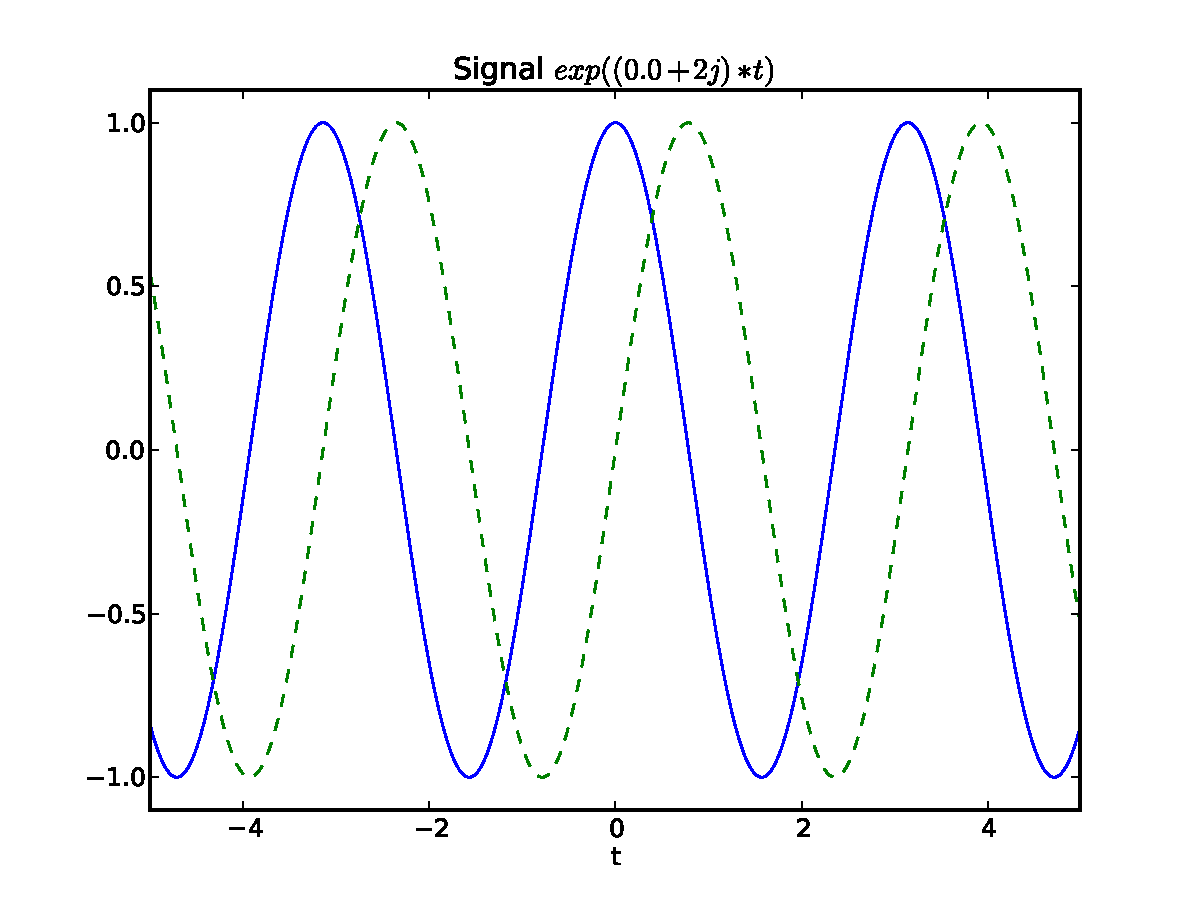
\includegraphics[width=.25\linewidth]{imgs/sig_conv/sig_exp01.pdf}\\
   \raisebox{9mm}{$.5$} 
    & 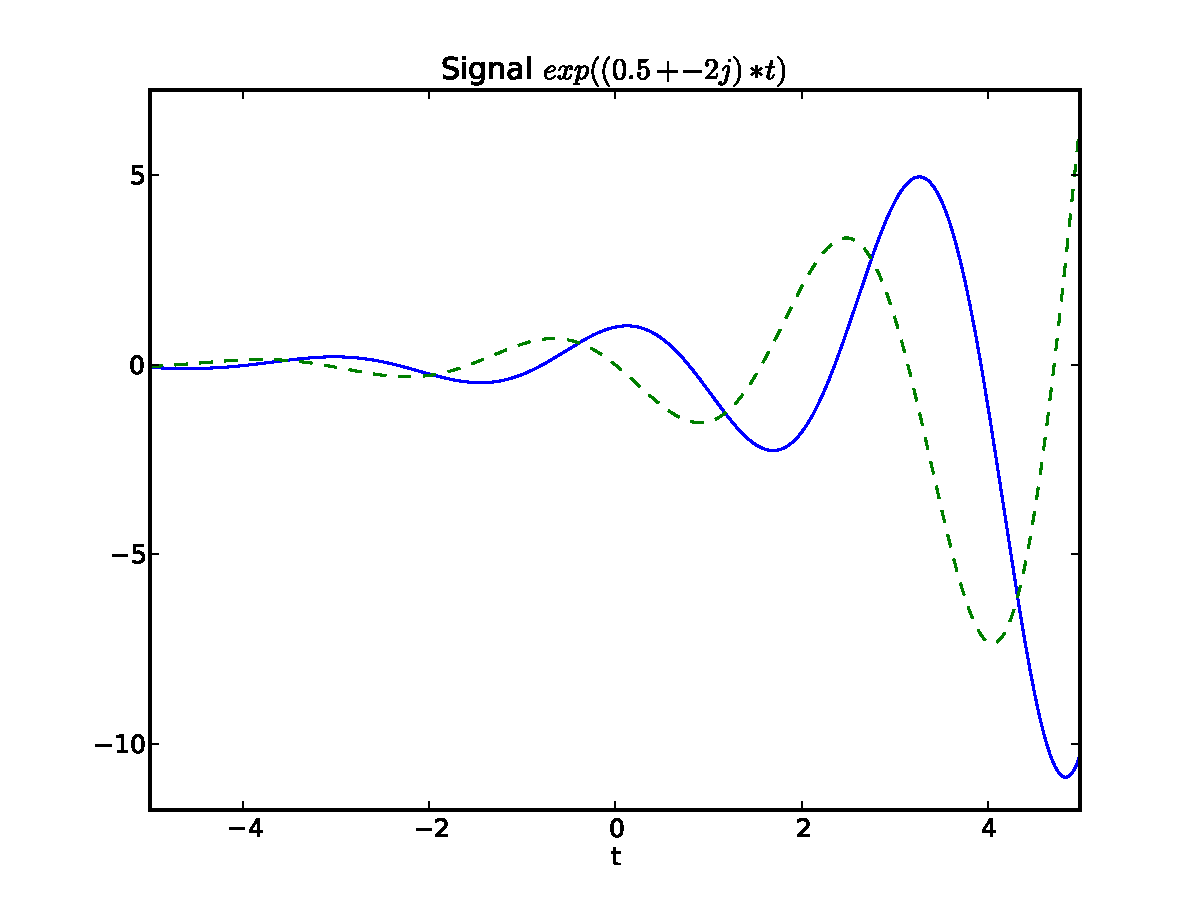
\includegraphics[width=.25\linewidth]{imgs/sig_conv/sig_exp1-1.pdf}
    & 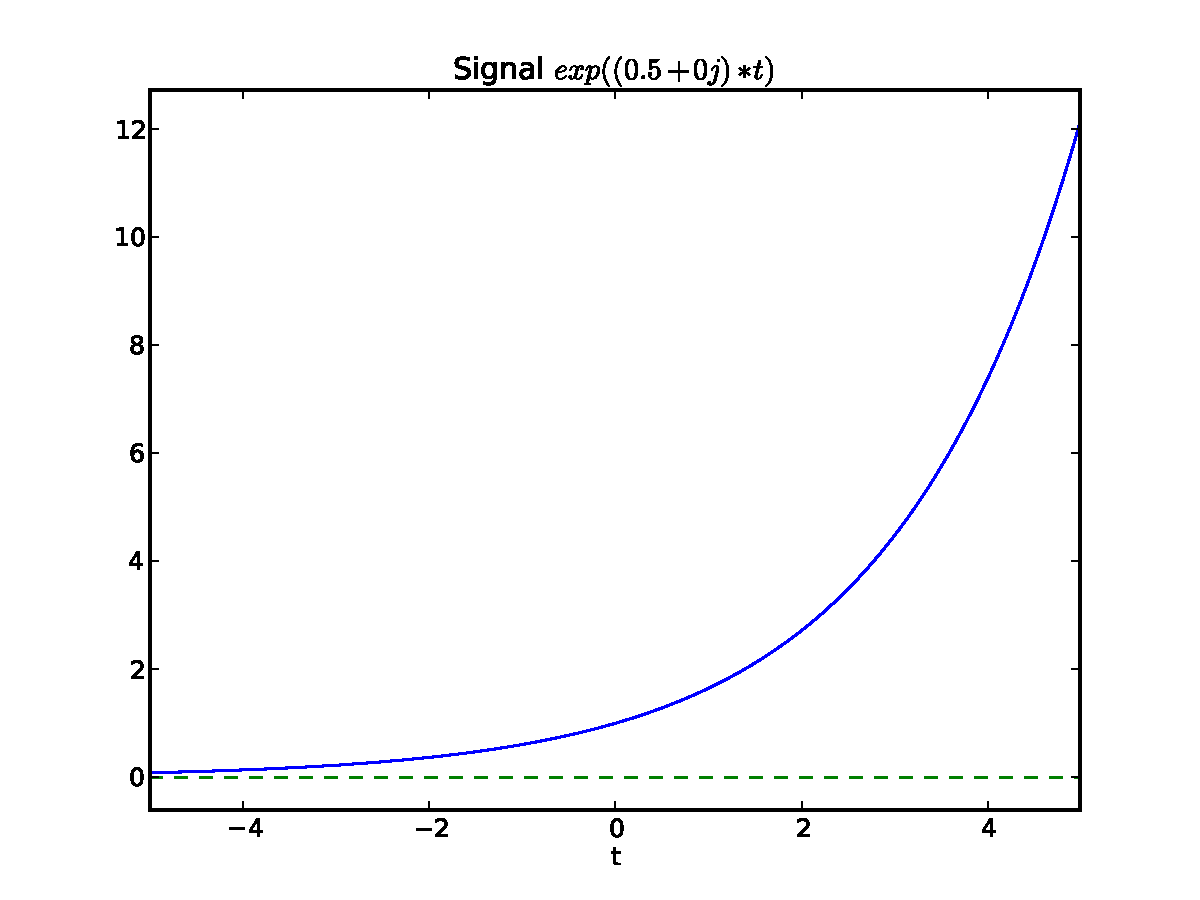
\includegraphics[width=.25\linewidth]{imgs/sig_conv/sig_exp10.pdf}
    & 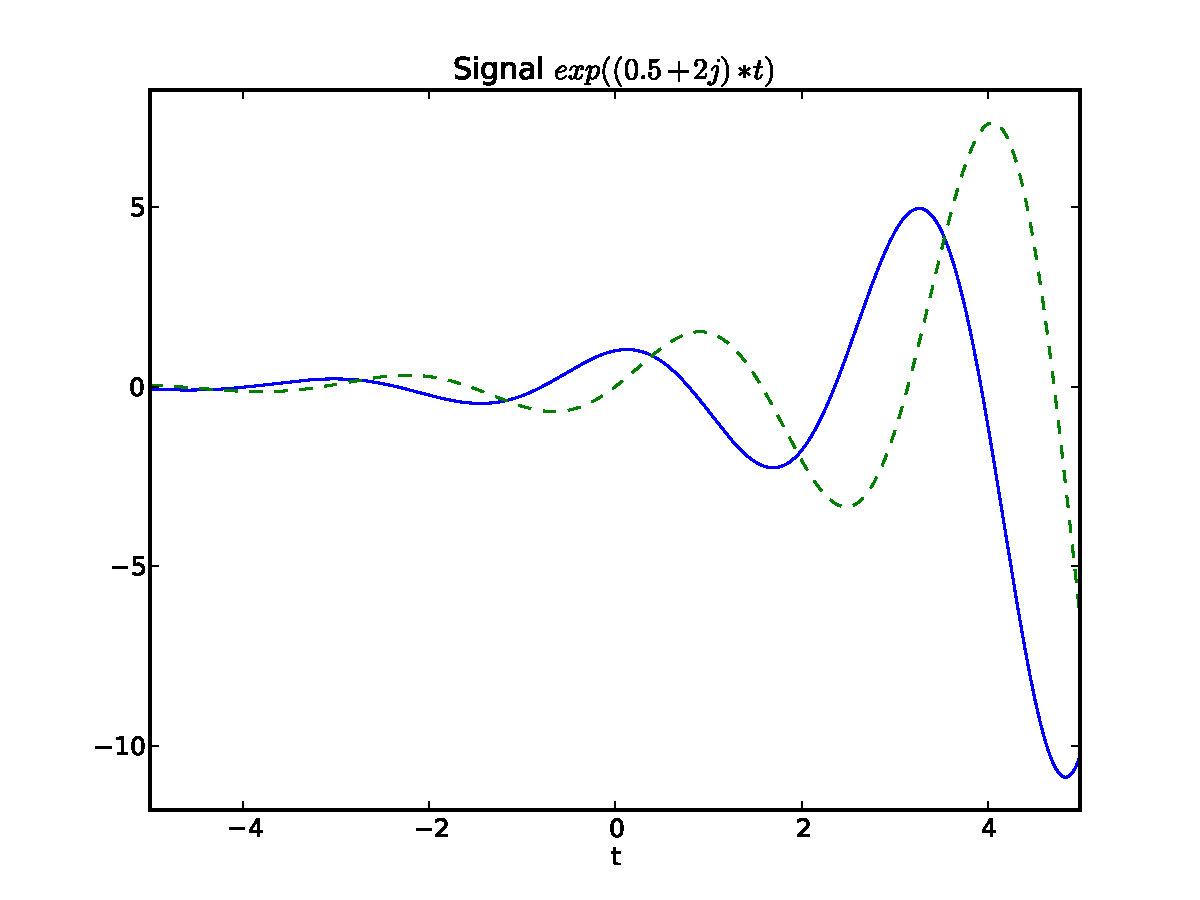
\includegraphics[width=.25\linewidth]{imgs/sig_conv/sig_exp11.pdf}\\
\hline
  \end{tabular}
  \caption{Example of complex exponential for different values of $z$}
  \label{fig:label}
\end{figure}

\subsubsection{Dirac delta}

\index{Dirac delta}

\begin{block}{Main properties of Dirac delta}


  \begin{itemize}
    \item Model point mass at $0$.
    \item Value outside $0$ :  $\delta(t)=0, \forall t\neq 0$ 
    %\item Can also be defined as $\lim_{T\rightarrow \infty} \Pi_T(t)$
    \item $\delta$ is a tempered distribution. % (not a function).
    \item Very useful tool in signal processing
   % \item All integrals with $\delta$ will be Lebesgue.
    \item Can be seen as the derivative of the Heavyside function $1_{t\geq 0}(t)$
    \item Integral
    \begin{equation}
      \label{eq:intdirac}
      \int_{-\infty}^{+\infty}\delta(t)dt=1 ,\qquad \int_{-\infty}^{+\infty}x(t)\delta(t)dt=x(0)
    \end{equation}
    \item Dirac and function evaluation for signal $x(t)$ and $t_0\in\R$ :
    %  $$ \delta(t)x(t)=\delta(t)x(0) $$
      $$\delta(t-t_0)x(t)=\delta(t-t_0)x(t_0) $$
   % \item Function evaluation :
    \begin{equation}
      \label{eq:diraceval}
      \langle  x(t) , \delta(t-t_0)\rangle=\int_{-\infty}^{+\infty}x(t)\delta(t-t_0)dt=x(t_0)
    \end{equation}
  
  \end{itemize}
  
  
  \end{block}

  \begin{block}{ Dirac delta definition}

    \begin{itemize}
      \item Let $\phi$ a function supported in $[-1,1]$ of unit mass: $\int_{-\infty}^\infty \phi(u)du=1$ 
      \item  $\phi_T(t)=\frac{1}{T}\phi(\frac{t}{T})$ has support on $[-T,T]$ and unit mass.
      \item We can define the dirac delta $\delta$ as
      $$ \delta(t)=\lim_{T\rightarrow 0} \phi_T(t) $$


    \end{itemize}
    
    
    \end{block}


    \begin{block}{Delta dirac in practice}
      \begin{itemize}
        \item Theoretical object in signal processing (impulse).
        \item Used to model signal sampling for digital signal processing.
        \item Used to model point source  in Astronomy/image processing, point charge in Physics.
        \item Has a bounded discrete variant.
      \end{itemize}
    \end{block}

    \subsection{Discrete time and digital signals}
    \label{sec:}
    

\section{Convolution and filtering}
\label{sec:conv_filtering}

\subsection{Convolution and properties}
\label{sec:}

\index{Convolution}.
\begin{block}{Convolution}
  Let two signals $x(t)$ and $h(t)$. The convolution between the two signals
  is defined as
  \begin{equation}
    x(t)\star h(t) =  \int_{-\infty}^{+\infty}x(\tau)h(t-\tau)d\tau
    \label{eq:convolution}
  \end{equation}\vspace{-5mm}
  \begin{itemize}
    \item Convolution is a bilinear mapping between $x$ and $h$.
    \item It models the relation between the input and the output of a Linear
    Time Invariant system.
    \item If $f\in L_1(\R)$ and $h\in L_p(\R), p\geq1$ then
    $$ \|f\star h\|_p\leq\|f\|_1\|h\|_p $$
    \item The dirac delta $\delta$ is the neutral element for the convolution operator:
\begin{equation}
      \label{eq:dirac_conv}
     x(t)\star \delta(t) =\int_{-\infty}^{+\infty}x(\tau)\delta(t-\tau)d\tau=  x(t)
    \end{equation}
    \begin{equation}
      \label{eq:dirac_conv_tz}
     x(t)\star \delta(t-t_0) = x(t-t_0)
    \end{equation}
 %   $$ x(t) * \delta(t) =  \int_{-\infty}^{+\infty}x(\tau)delta(t-\tau)d\tau=x(t)$$
  \end{itemize}

\end{block}


\paragraph{Example of convolution}
 
% figure in latex, video in HTML
\begin{warpHTML}
  \begin{figure}[ht]
    \centering
    <video width="671" height="472" controls>
    <source src="imgs/sig\_conv/movie\_conv.mp4" type="video/mp4">
    <source src="imgs/sig\_conv/movie\_conv.webm" type="video/webm">
    Your browser does not support the video tag.
    </video>   
    \caption{Illustration of the convolution operator between the Heaviside step function and a causal decreasing exponential.}
    \label{fig:convolution}
  \end{figure}
\end{warpHTML}
\begin{warpprint}
  \begin{figure}[ht]
    \centering
    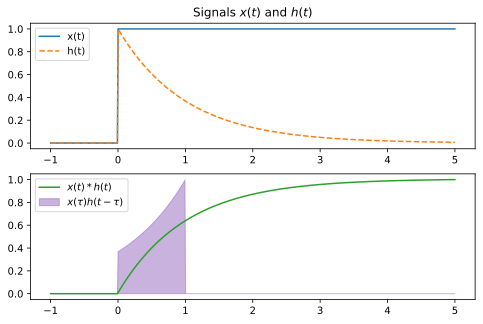
\includegraphics[width=.7\linewidth]{imgs/sig_conv/signals_conv}
    \caption{Illustration of the convolution operator between the Heaviside step function and a causal decreasing exponential.}
    \label{fig:convolution}
  \end{figure}
\end{warpprint}
%\begin{center}
  %\only<1>{ 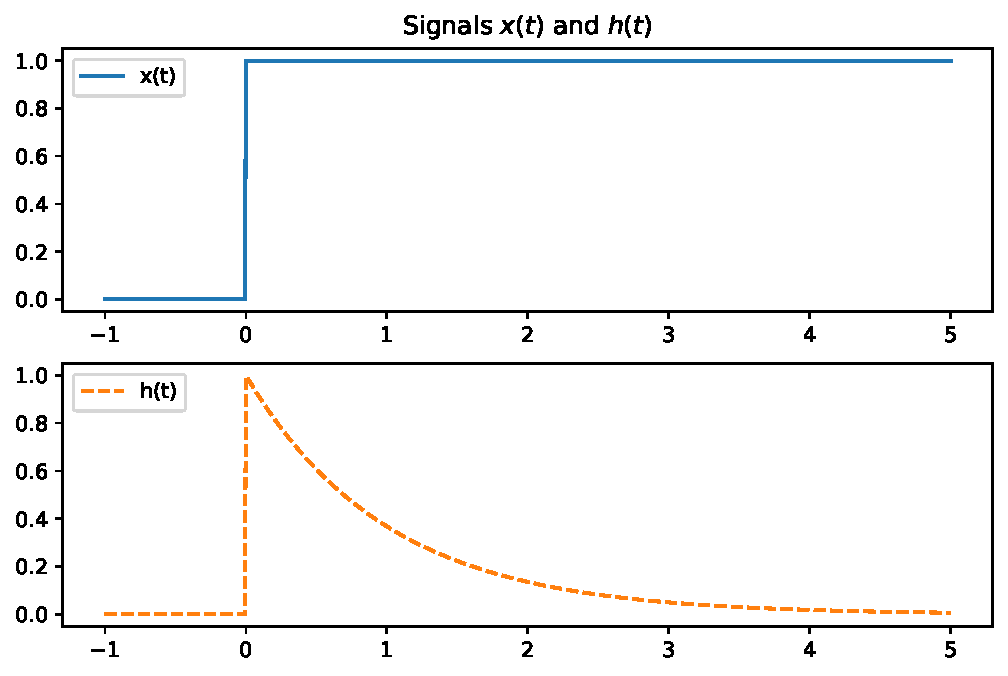
\includegraphics[width=.64\linewidth]{imgs/conv_demo/signals}}

 % \only<2>{ \inlineMovie{imgs/conv_demo/movie.mp4}{imgs/conv_demo/conv_000}{width=.64\linewidth}}
%\only<3>{ 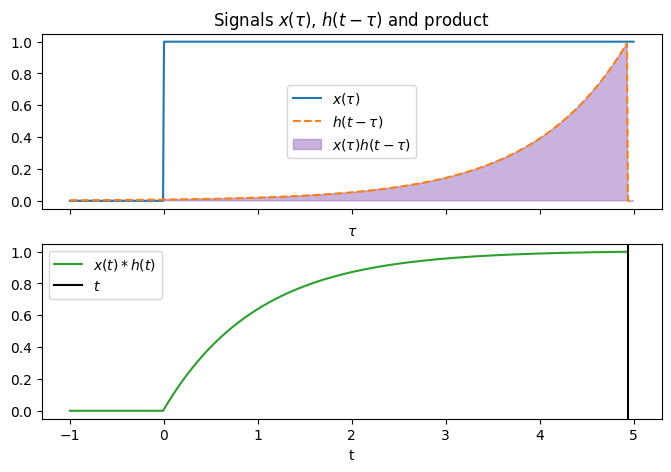
\includegraphics[width=.64\linewidth]{imgs/conv_demo/conv_098}}


\begin{itemize}
\item $x(t)=\Gamma(t)$ the Heaviside step function.
\item $h(t)=e^{-t}\Gamma(t)$ the positive part of the decreasing exponential.
\item $x(t)\star h(t)=(1-e^{-t})\Gamma(t)$
\end{itemize}

\subsection{Linear Time Invariant (LTI) systems}
\label{sec:lti_systeùs}



\section{Discrete time and digital signals}
\label{sec:def_disrete_signal}

\subsection{Discrete time}

\subsection{Finite signals}
\label{sec:finite}

\subsection{Quantization and storage}
\label{sec:}


\section{Fundamental signal processing problems}
\label{sec:sp_prob}

\subsection{Filtering}


\subsection{Deconvolution, unmixing and regression}


\subsection{Blind source separation and deconvolution}



